\documentclass{article}
\usepackage[preprint]{neurips_2026}
\usepackage[T1]{fontenc}
\usepackage[utf8]{inputenc}
\usepackage{microtype,booktabs,amsmath,amssymb}
\usepackage[table]{xcolor}
\definecolor{MuSage}{HTML}{B7D7C0}
\definecolor{MuLavender}{HTML}{C9C0E8}
\definecolor{MuApricot}{HTML}{E8C6AA}
\definecolor{MuCream}{HTML}{FAF8F2}
\definecolor{MuForest}{HTML}{28483D}
\usepackage{tikz}
\usetikzlibrary{arrows.meta,positioning}
\usepackage[colorlinks=true,linkcolor=MuForest,citecolor=MuForest,urlcolor=MuForest]{hyperref}
\hypersetup{pdftitle={MuDuSi: A Multi-Agent Acoustic Simulator for Full-Duplex Speech Language Models},pdfauthor={Kyudan Jung; Jaegul Choo},pdfsubject={Technical Report MUDUSI-TR-2026-01, Version 1.0, October 12, 2026},pdfkeywords={full-duplex speech, multi-agent simulation, acoustic trajectories, reinforcement learning}}
\title{MuDuSi: A Multi-Agent Acoustic Simulator\\ for Full-Duplex Speech Language Models}
\author{Kyudan Jung \qquad Jaegul Choo\\KAIST AI\\[3pt]
Technical Report MUDUSI-TR-2026-01\\October 12, 2026\quad$\cdot$\quad Version 1.0\\
\url{https://kyudan1.github.io/MuDuSi/paper/}}
\newcommand{\code}[1]{\texttt{#1}}
\begin{document}
\maketitle
\begin{abstract}
MuDuSi (Multi-agent Duplex Simulator) is a virtual acoustic testbed for independently running full-duplex speech models. It couples simultaneous listening and speaking through a 24 kHz PCM engine with distance-dependent attenuation, propagation delay, occlusion, reflection, and microphone noise, and visualizes their interaction in a shared 3D scene. The same engine supports frozen-model conversation evaluation and acoustic trajectory collection for reinforcement-learning research. We describe its timing and recording contracts and report bounded NVIDIA B200 experiments with PersonaPlex, Moshi, and Raon. Two 60-second PersonaPlex--Moshi runs completed at wall-clock rate with zero input overflows or dropped output samples; recorded model inputs exactly matched the preceding receiver blocks after PCM16 encoding. Additional two- and three-agent runs demonstrate concurrent generated speech and role-conditioned interaction. These results establish execution and routing feasibility, not semantic task performance. We distinguish acoustic trajectories from token-policy rollouts, document observed dialogue and synthesis failures, and identify the interfaces required for speech-model reinforcement learning.
\end{abstract}

\section{Introduction}
Full-duplex speech models can listen while speaking, producing overlaps, backchannels, and interruptions that alternating-turn text harnesses cannot represent directly. In a shared room, each participant also hears a different signal: distance, occlusion, and noise transform the sound emitted by other participants. Studying these interactions with physical devices can require a separate microphone/loudspeaker setup for each agent and repeated room configuration.

MuDuSi provides a software testbed before such deployment. Independent model sessions exchange audio through a common acoustic engine, while a 3D observer exposes source activity, local microphone mixtures, and timing. Its two workflows are frozen-model inference/evaluation and acoustic trajectory collection for reinforcement-learning (RL) research. Recorded experiments can be replayed without keeping GPUs allocated. This reduces dependence on physical devices for software experiments, but does not replace hardware or perceptual validation.

The contribution is an executable interaction substrate: simultaneous PCM actions, explicit receiver-to-input alignment, bounded asynchronous transport, and inspectable audiovisual records. We report engineering measurements from real model runs rather than a semantic benchmark. Full-weight speech-language model (SLM) RL is not implemented; the included trainable example is a small stochastic gate. The code and operational records are available at \url{https://github.com/KyuDan1/MuDuSi}.

\section{Related work}
\paragraph{Speech models.} Moshi jointly models incoming and outgoing speech streams, with time-aligned text generation \citep{defossez2024moshi}. PersonaPlex adds role and voice conditioning to a Moshi-derived full-duplex model \citep{roy2026personaplex}. MuDuSi connects independent instances of such models through spatial microphone mixtures; it does not propose a new speech architecture. Whisper \citep{radford2023whisper} is used as an external recognizer, with its output kept separate from native model text.

\paragraph{Simulation and multi-agent interfaces.} MuJoCo supplies a physics engine designed for model-based control \citep{todorov2012mujoco}. MuDuSi shares the motivation of testing interacting policies in simulation, but models acoustic exchange rather than rigid-body/contact dynamics and does not use MuJoCo as its backend. PettingZoo standardizes multi-agent environment interaction \citep{terry2020pettingzoo}; MuDuSi's parallel dictionaries follow a similar interface convention, without claiming PettingZoo registration or compliance.

\paragraph{Acoustic environments.} Pyroomacoustics provides room impulse-response simulation and audio-array processing tools \citep{scheibler2017pyroomacoustics}. SoundSpaces supplies geometrical acoustic renderings for audio-visual navigation in 3D environments \citep{chen2020soundspaces}. MuDuSi's present acoustics are deliberately simpler. Its focus is the closed interaction loop between independently stateful speech generators, live buffer diagnostics, and aligned source/receiver/input recordings. Neither richer room simulation nor spatial visualization alone establishes a validated speech-agent benchmark.

\section{Method: the simulation and recording contract}
\begin{figure}[t]
\centering
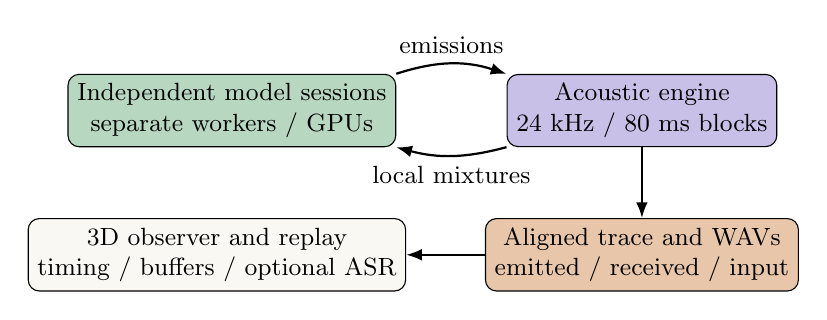
\begin{tikzpicture}[font=\small,box/.style={draw,rounded corners,align=center,minimum height=9mm},arr/.style={-{Latex[length=2mm]},thick}]
\node[box,fill=MuSage] (a) {Independent model sessions\\separate workers / GPUs};
\node[box,fill=MuLavender,right=14mm of a] (b) {Acoustic engine\\24 kHz / 80 ms blocks};
\node[box,fill=MuApricot,below=9mm of b] (c) {Aligned trace and WAVs\\emitted / received / input};
\node[box,fill=MuCream,left=10mm of c] (d) {3D observer and replay\\timing / buffers / optional ASR};
\draw[arr] (a.north east) to[bend left=18] node[above]{emissions} (b.north west);
\draw[arr] (b.south west) to[bend left=15] node[below]{local mixtures} (a.south east);
\draw[arr] (b)--(c);\draw[arr] (c)--(d);
\end{tikzpicture}
\caption{All sessions may emit and receive concurrently. The observer does not drive simulation time. Clean source audio is available for analysis, not substituted for a peer's microphone input.}
\end{figure}

\subsection{Acoustic dynamics and timing}
The engine accepts simultaneous mono float32 emissions of $B=1{,}920$ samples at $f_s=24{,}000$ Hz, an 80 ms decision interval. Policies consume the previous completed receiver block; current emissions jointly determine the next observations. Initial model input is silence. For source $i$ and receiver $j$, direct pressure gain and delay are
\begin{align}
 g_{ij}&=\frac{1}{\max(1,d_{ij})}\prod_{k\in\mathcal O_{ij}}10^{-L_k/20},\qquad
 \tau_{ij}=\left\lceil d_{ij}f_s/343\right\rceil,
 \\
 y_j[n]&=\sum_{i\ne j}g_{ij}x_i[n-\tau_{ij}]+r_j[n]+\epsilon_j[n].
\end{align}
Here $d_{ij}$ is distance in meters, $L_k$ is an intersected divider's loss in dB, and $\epsilon_j$ is independent Gaussian microphone noise with RMS $10^{\eta/20}$. There is no own-source path. Delay queues cross block boundaries. Geometry is evaluated at emission time, so moving an agent does not rewrite sound already in flight. The optional $r_j$ is one right-wall image-source reflection with gain $0.45\rho/\max(1,d^{\mathrm{refl}}_{ij})$. The reflection control $\rho$ is not a calibrated RT60. Raw superposition remains unclipped; WAV encoding and live inputs clamp to $[-1,1]$ and expose clipping counters.

Headless CPU steps advance without wall-clock pacing. Live evaluation instead uses a paced 80 ms clock and independent asynchronous worker send/receive loops. Bounded queues expose underruns, overflow, dropped samples, and final queued audio. Slow observers lose stale visual updates rather than backpressuring the acoustic loop. Physical propagation, block decision delay, codec buffering, and model inference are distinct latency sources. A fixed acoustic seed does not make asynchronous GPU trajectories bitwise reproducible.

\subsection{Inference, trajectories, and visualization}
Each participant has a separate endpoint and model state. Two or three workers can converse in one scene; a WAV worker can instead provide controlled stimulation. The current engine has three named slots, not arbitrary agent counts. Multiple independent experiments require separate evaluator processes and output directories; the viewer is not a multi-scene scheduler.

The evaluator saves one JSONL snapshot per tick and three PCM16 WAVs per slot: emitted audio at the mixer boundary, the spatially mixed receiver signal, and the previous receiver block supplied to the adapter. Summaries preserve completion/failure, elapsed time, scheduler lateness, and final diagnostics. Partial failures remain identifiable. This same evaluator supplies an acoustic trajectory; there is no separate token-rollout mode.

The parallel Python environment returns each agent's microphone PCM, own position, and time, plus acoustic rewards and boundary flags. All agents act simultaneously. A fixed horizon is truncation, not natural task termination. Rewards combine source-attributed audibility, an overlap penalty, and emission energy. They are development proxies: useful backchannels may incur a penalty, and audibility is not comprehension. A four-parameter Bernoulli listen/speak gate illustrates REINFORCE \citep{williams1992simple}, logging behavior probabilities and policy versions with parameters frozen during each rollout. It emits synthetic tones and does not update SLM weights.

The 3D viewer shows transmitted and received RMS, activity, propagation labels, and buffer timing. dBFS is not calibrated sound pressure, and activity is a $-65$ dBFS energy detector. Animated wave rings deliberately slow apparent propagation. Engineering replay plays actual receiver audio; presentation videos mix clean emissions for intelligibility. Their speech bubbles are offline Whisper ASR on emitted audio, revealed at word timestamps, not native text or measured streaming-ASR latency.

\section{Experiments and results}
\subsection{Setup and measurements}
Experiments ran on NVIDIA B200 GPUs (183,359 MiB each), driver 580.95.05, using isolated Slurm allocations. Paired runs requested two GPUs, 16 CPUs, and 96 GiB RAM; each model occupied one GPU. PersonaPlex and Moshi used separate Python environments because both install a package named \code{moshi}. The exercised model paths used Torch 2.8.0/CUDA 12.8 and an NVIDIA PyTorch 25.04 worker image for runtime compilation. PersonaPlex's reused environment had dependency conflicts outside the tested inference path; successful runs do not certify that entire environment.

Two 60-second (750-frame) PersonaPlex--Moshi experiments used the same spoken rice-cooking WAV stimulus in the third slot. The near condition used 1 m model separation, no divider, and $-72$ dBFS microphone noise. The distant condition used 5.70 m separation, a 14 dB divider, and $-35$ dBFS noise. These jointly changed factors are not an acoustic ablation. We measured pacing, buffer health, activity overlap, and source/receiver/input consistency. Timing starts after worker readiness, excluding startup and scheduling.

\begin{table}[t]
\centering
\caption{Measured paired conversations. Overlap counts the two models, excluding the stimulus. Handler timing is not end-to-end response latency.}
\label{tab:pair}
\begin{tabular}{lrr}\toprule
\rowcolor{MuCream}
Measurement & Near / quiet & Distant / cocktail\\\midrule
Slurm job & 189794 & 189798\\
Audio / wall duration (s) & 60 / 60.011 & 60 / 60.007\\
Scheduler lateness, p95 (ms) & 1.45 & 2.04\\
Tick overruns / input overflow / dropped samples & 0 / 0 / 0 & 0 / 0 / 0\\
PersonaPlex / Moshi startup underrun frames & 1 / 2 & 1 / 2\\
Moshi handler mean / p95 (ms) & 24.59 / 26.15 & 24.19 / 26.20\\
Both models active (s) & 3.12 & 6.56\\
Direct model-to-model pressure gain (dB) & 0 & $-29.12$\\\bottomrule
\end{tabular}
\end{table}

\subsection{Routing and runtime evidence}
For every receiver in both runs, recorded input at tick $t$ exactly matched PCM16-encoded received audio at $t-1$, with initial silence. Re-rendering saved emissions through the mixer reproduced received WAVs within maximum normalized amplitude errors of $9.2\times10^{-5}$ and $4.5\times10^{-5}$, respectively; the small discrepancies reflect source/WAV quantization. This verifies delivery to the adapter, with native transport encoding remaining a separate codec stage.

Both experiments completed at wall-clock rate (Table~\ref{tab:pair}), with no counted ADC or decoder clipping. Underruns occurred before initial generated samples arrived; buffers were not prefilled. One 80 ms block remained queued at the fixed endpoint. Near-run monitoring reported approximately 17,839 MiB for Moshi and 19,625 MiB for PersonaPlex, 36.4 GiB host working memory, and no OOM or CPU throttling. These are sampled readings, not allocator peaks or training-memory estimates. Paced completion does not measure maximum throughput.

Receiver ASR recognized cooking-answer content in the peer's microphone recording. The second stimulus began while Moshi spoke, with overlap and later stop/resume visible in the traces. This establishes an interruption stimulus and activity, not causal intentional yielding. Noisy receiver ASR also hallucinated repetitions; neither recognition nor native text is ground-truth comprehension.

\subsection{Model-only conversations and failure cases}
Additional runs used no prerecorded speaker (Table~\ref{tab:showcase}). The cafe workers received clerk/customer roles, voice prompts, and menu context, not scripted dialogue. The selected passage contains an iced oat-latte and croissant order and confirmation. The full run includes initial role confusion and an incorrect price. Longer friends and three-agent conversations contain monologues and repetitive backchannels; selecting favorable clips introduces selection bias.

\begin{table}[t]
\centering
\caption{Additional independent conversations; all had zero input overflow, output drops, and clipping. Three participants comprise two model families.}
\label{tab:showcase}
\begin{tabular}{lrrr}\toprule
\rowcolor{MuCream}
 & Friends & Clerk / customer & Three agents\\\midrule
PersonaPlex / Moshi instances & 1 / 1 & 2 / 0 & 2 / 1\\
Slurm job & 189846 & 189891 & 189845\\
Full recording (s) & 90 & 60 & 90\\
Scheduler lateness, p95 (ms) & 1.57 & 1.69 & 1.26\\
Startup underrun frames & 1 + 2 & 1 + 1 & 1 + 2 + 1\\
Selected interval (s) & 0--26.92 & 9.50--30.25 & 0--14.92\\\bottomrule
\end{tabular}
\end{table}

All connected model inputs matched their previous receiver blocks. Full-run overlap measured 10.96 s for friends and 48.08 s for three agents; the selected intervals contain 3.76 s and 6.96 s. These are activity statistics, not dialogue-quality scores.

The direct Raon PyTorch bridge generated audio/text but averaged 207 ms per 80 ms frame and filled its 32-frame input queue after 4.24 simulated seconds (job 189796). An optimized SGLang path, after CUDA runtime/library-path fixes, completed 60 s in 60.012 s with 1.68 ms p95 lateness and zero overflow/drops (job 189820). Raon had six startup underrun frames and 480 ms queued at the endpoint. Monitoring reported about 90,085 MiB for Raon, including preallocated cache. A warmup mismatch and missing intended sliding-window behavior in an attention fallback remained. Later generated audio diverged substantially from native text and contained garbled phrases. These are unresolved quality failures; the warnings are candidate causes, not established causal explanations.

\section{Limitations and research directions}
The current acoustics use three slots, quadratic source--receiver paths, nondirectional mono signals, and a single reflection. There is no validated room impulse response, HRTF, calibrated SPL, or physical loudspeaker feedback loop. The execution record contains a small number of stochastic episodes without repeated-seed confidence intervals, human intelligibility labels, or controlled counterfactual interruption trials. Changed acoustics also change downstream model actions, preventing isolated causal attribution. Selected demonstrations and low scheduler lateness cannot establish semantic performance.

Diarization-capable models could consume mixed receiver audio through suitable adapters, but no diarization-specific output contract, identity metric, or verified result is implemented. Known source IDs and caption labels are provenance, not inferred speaker identities. Such evaluation requires timestamped predicted speakers, receiver-aligned reference activity, and overlap-aware scoring. More agents, vectorized scenes, and richer acoustics also require implementation beyond the present viewer.

Full SLM RL requires sampled text/audio-code token IDs, behavior log-probabilities under the actual sampling distribution, valid-action masks, policy/checkpoint versions, reset boundaries, and token-to-PCM timing. A critic additionally needs aligned values; privileged critic features must remain separate from actor inputs. Version barriers must finish or discard old-policy episodes before publishing new weights. The next step is an instrumented frozen worker with probability recomputation, followed by a bounded adapter/LoRA update and held-out evaluation. Acoustic recordings or ASR reconstruction alone are insufficient to claim an on-policy SLM update.

\section{Conclusion}
MuDuSi provides a virtual shared acoustic space for independent full-duplex speech sessions, with observable timing and aligned trajectories. B200 runs verify paced execution and the route from model emissions to peer adapter inputs. Dialogue failures, Raon synthesis degradation, simplified acoustics, and missing token-policy interfaces limit broader claims. The simulator supplies a practical foundation for controlled conversation evaluation and future RL integration, while keeping those engineering capabilities distinct from demonstrated conversational competence.

\paragraph{Reproducibility and release.}
This self-published MuDuSi Project technical report documents the experiments above, whose original implementation is recorded at revision \code{4e4f0f4}. The repository's B200 verification and showcase documents retain job provenance, model revisions, rerun commands, and limitations. Generic configurations, tests, and report sources are public; weights, credentials, private settings, and large raw recordings are excluded. Generated audio and caption provenance should remain labeled, with model licenses and voice permissions respected. This report uses the NeurIPS 2026 preprint format and makes no claim of conference submission or acceptance.

\clearpage
\bibliographystyle{plainnat}
\bibliography{mudusi-technical-report}
\end{document}
